%==============================================================================
% sections/03_independent_baseline.tex
%==============================================================================
\section{Independent Baseline}
\label{sec:independent-baseline}

This section records the independent theory inherited from the original
manuscript. It is included because every dependent extension is easiest to
understand by comparing its tail constant and estimator with the independent
benchmark.

\subsection{Maximum and sum asymptotics}

\begin{assumption}[Independent pointwise tail equivalence]
\label{ass:ind-pte}
The random variables \(X_1,\ldots,X_N\) are independent, \(N<\infty\), and
there exists \(\Gb\in\RV_{-\alpha}\), \(\alpha>0\), such that
\[
  \Pb(X_i>x)\sim c_i\Gb(x), \qquad i=1,\ldots,N.
\]
At least one \(c_i\) is positive.
\end{assumption}

\begin{theorem}[Exact leading maximum asymptotic]
\label{thm:catastrophe-exact}
Under \cref{ass:ind-pte},
\[
  \Pb(M_N>x)
  = \sum_{i=1}^N\Pb(X_i>x)+o(\Gb(x))
  \sim C\Gb(x).
\]
\end{theorem}

\begin{proof}[Proof sketch]
Finite inclusion--exclusion: pair intersections are products of marginal tails,
hence $O(\Gb(x)^2)=o(\Gb(x))$, and there are finitely many pairs. The full
argument appears in \cref{appx:independent-proofs}.
\end{proof}

The exact constant is \(C\), with no slack factor.

For sums, marginal right-tail equivalence alone is insufficient because large
negative components could cancel a large positive component and because many
moderate components could combine to cross \(x\). The usual finite-dimensional
single-big-jump truncation conditions rule out those pathologies.

\begin{assumption}[Independent finite-sum single-big-jump conditions]
\label{ass:ind-sbj}
In addition to \cref{ass:ind-pte}, the left tails are negligible at the right
reference scale and there exists \(h(x)\uparrow\infty\), \(h(x)=o(x)\), such
that for each active \(i\),
\[
  \Pb(X_i>x-h(x))\sim \Pb(X_i>x),
\]
and the probability that two or more truncated components exceed order \(h(x)\)
is \(o(\Gb(x))\). Equivalently, the finite collection is in the one-large-jump
subexponential regime used for the displayed sum equivalence.
\end{assumption}

\begin{theorem}[Independent sum equivalence]
\label{thm:sum-equivalence}
Under \cref{ass:ind-sbj},
\[
  \Pb(S_N>x)
  \sim \sum_{i=1}^N\Pb(X_i>x)
  \sim C\Gb(x).
\]
\end{theorem}

\begin{proof}[Proof sketch]
A truncation argument combined with the pair-exceedance estimate of
\cref{thm:catastrophe-exact}. The full upper and lower bounds appear in
\cref{appx:independent-proofs}.
\end{proof}

%==============================================================================
% figures/F1_tail_equivalence.tex --- Implementation placeholder
%==============================================================================
% Required source CSV: results/F1_tail_equivalence.csv
% Required columns: seed, spawned_seed, N, alpha, x, n, mu_hat, ci_low, ci_high, first_order, second_order, truth_method
% Target diagnostic: Plot log-log tail estimates against first- and second-order asymptotics.
% Replacement instruction:
%   Generate a PDF/PNG with the same basename and replace the tikzpicture below
%   by 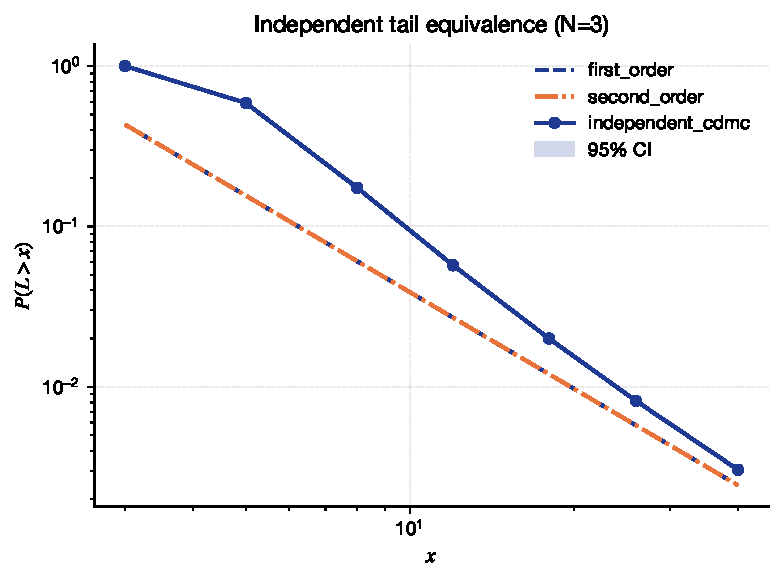
\includegraphics[width=0.85\linewidth]{figures/F1_tail_equivalence.pdf}.
%==============================================================================
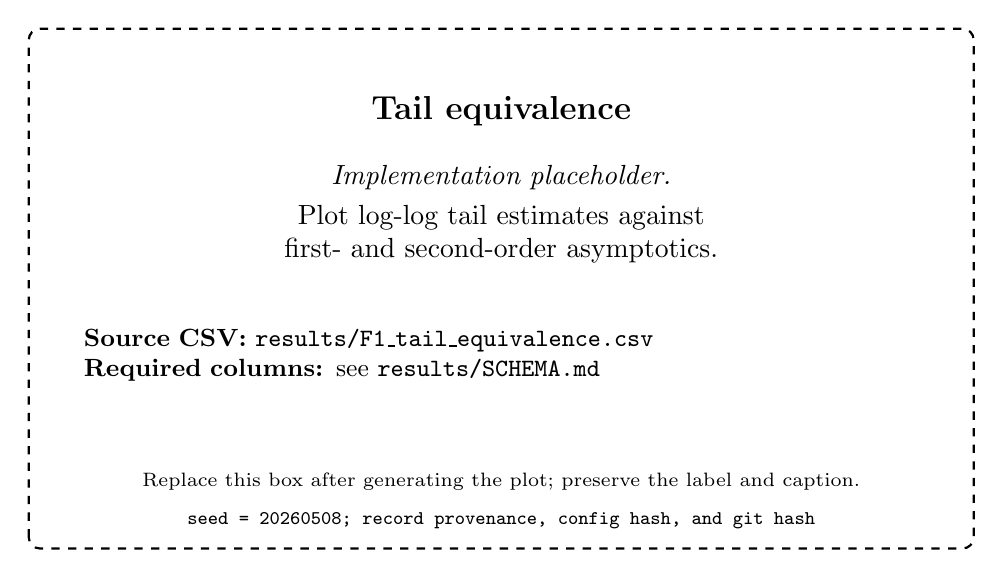
\begin{tikzpicture}
\draw[thick, dashed, rounded corners] (0,0) rectangle (12,6.6);
\node[align=center, font=\large] at (6,5.55) {\textbf{Tail equivalence}};
\node[align=center, text width=10.6cm] at (6,4.25) {\emph{Implementation placeholder.}\\[0.25em]
Plot log-log tail estimates against first- and second-order asymptotics.};
\node[align=left, text width=10.6cm, font=\small] at (6,2.45) {\textbf{Source CSV:} \texttt{results/F1\_tail\_equivalence.csv}\\
\textbf{Required columns:} see \texttt{results/SCHEMA.md}};
\node[align=center, font=\scriptsize] at (6,0.85) {Replace this box after generating the plot; preserve the label and caption.};
\node[align=center, font=\scriptsize\ttfamily] at (6,0.35) {seed = 20260508; record provenance, config hash, and git hash};
\end{tikzpicture}


\Cref{fig:ind-tail-equivalence} demonstrates
\cref{thm:catastrophe-exact,thm:sum-equivalence} empirically: the
independent CdMC estimator sits between the first-order line and the
second-order curve, and converges to the first-order line in the deep
tail. The catastrophe principle itself --- the ratio
$P(M_N > x) / P(S_N > x) \to 1$ --- is verified separately in
\cref{fig:max-vs-sum}.

\subsection{Corrected second-order expansion}

The second-order term is important for finite thresholds. When \(X_i\) is the
large component, the first-order shift is created by the remaining sum
\(S_{-i}\), not by \(X_i\) itself. This yields the leave-one-out mean.

\begin{assumption}[Second-order tail equivalence and finite means (independent baseline)]
\label{ass:sote-ind}
The active variables satisfy the local second-order condition
\cref{ass:sote}; \(\E|X_i|<\infty\) for all \(i\); and inactive or lighter-tail
summands are negligible at scale \(\Gb(x)(|A(x)|\vee x^{-1})\).
\end{assumption}

\begin{theorem}[Second-order independent expansion]
\label{thm:second-order}
Under \cref{ass:ind-sbj,ass:sote-ind},
\[
  \Pb(S_N>x)
  = C\Gb(x)
    + \Gb(x)A(x)\sum_{i\in\Aset}c_id_i
    + \frac{\alpha\Gb(x)}{x}\sum_{i\in\Aset}c_i\mu_{-i}
    + o\{\Gb(x)(|A(x)|\vee x^{-1})\},
\]
where \(\mu_{-i}=\sum_{j\ne i}\E X_j\).
\end{theorem}

\begin{proof}[Proof sketch]
Stratify by the selected-maximum index from \cref{ass:tie}, localize to
\(|S_{-i}|\le h(x)\), and apply the second-order tail equivalence of
\cref{ass:sote} term by term. The full expansion, including the localization
and inactive-component bounds, appears in \cref{appx:independent-proofs}.
\end{proof}

The formula passes the \(N=1\) check because \(\mu_{-1}=0\); a Lomax/Pareto
benchmark verifies the cross-term by direct substitution (see
\cref{appx:independent-proofs}, verification notes). The constants can be
written in closed form and used as a regression test for implementations.

%==============================================================================
% figures/F8_second_order.tex --- Implementation placeholder
%==============================================================================
% Required source CSV: results/F8_second_order.csv
% Required columns: seed, spawned_seed, x, mu_hat, first_order, second_order, normalized_error, target_constant, n_equals_one_check
% Target diagnostic: Check the corrected Lomax second-order constant and N=1 sanity test.
% Replacement instruction:
%   Generate a PDF/PNG with the same basename and replace the tikzpicture below
%   by 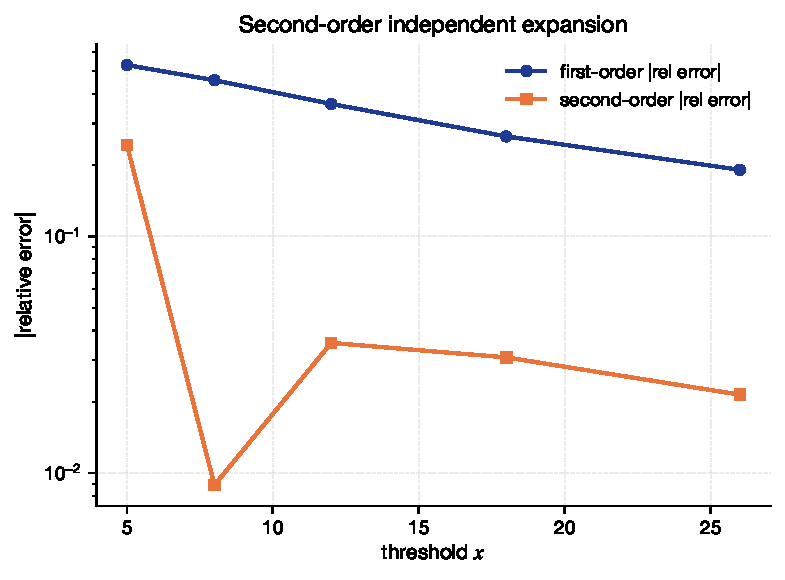
\includegraphics[width=0.85\linewidth]{figures/F8_second_order.pdf}.
%==============================================================================
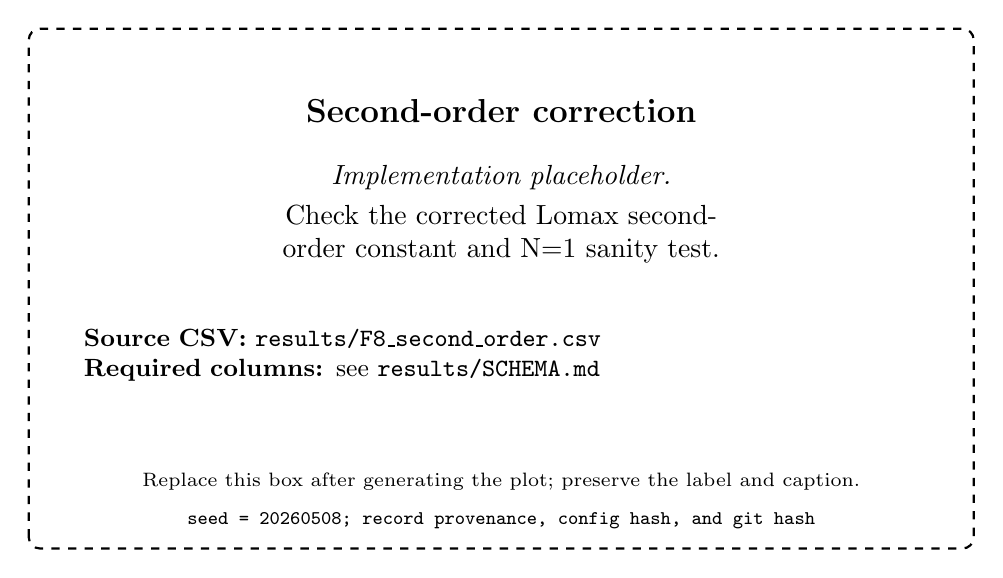
\begin{tikzpicture}
\draw[thick, dashed, rounded corners] (0,0) rectangle (12,6.6);
\node[align=center, font=\large] at (6,5.55) {\textbf{Second-order correction}};
\node[align=center, text width=10.6cm] at (6,4.25) {\emph{Implementation placeholder.}\\[0.25em]
Check the corrected Lomax second-order constant and N=1 sanity test.};
\node[align=left, text width=10.6cm, font=\small] at (6,2.45) {\textbf{Source CSV:} \texttt{results/F8\_second\_order.csv}\\
\textbf{Required columns:} see \texttt{results/SCHEMA.md}};
\node[align=center, font=\scriptsize] at (6,0.85) {Replace this box after generating the plot; preserve the label and caption.};
\node[align=center, font=\scriptsize\ttfamily] at (6,0.35) {seed = 20260508; record provenance, config hash, and git hash};
\end{tikzpicture}


The corrected expansion reduces the absolute relative error of the
leading sum-tail approximation by roughly an order of magnitude across
the threshold range (\cref{fig:second-order-placeholder}). The
$N=1$ check is mechanical: when there is a single summand the
leave-one-out sum is empty and the second-order term vanishes,
recovering the standard single-variable second-order tail asymptotic.

\subsection{Independent conditional Monte Carlo}

For independent variables define
\[
  Z^{\mathrm{ind}}(x)=\sum_{i=1}^N \Fb_i(T_i(x)),
  \qquad \Fb_i(t)=\Pb(X_i>t).
\]
The selected-maximum events partition \(\{S_N>x\}\), and independence gives
\(\Pb(X_i>T_i\mid X_{-i})=\Fb_i(T_i)\). Thus \(Z^{\mathrm{ind}}\) is unbiased.
Moreover \(T_i(x)\ge x/N\) on the relevant scale, so
\[
  0\le Z^{\mathrm{ind}}(x)\le B(x):=\sum_{i=1}^N\Fb_i(x/N).
\]
Since \(B(x)/\mu(x)\to N^\alpha\),
\[
  \limsup_{x\to\infty}
  \frac{\Var(Z^{\mathrm{ind}}(x))}{\mu(x)^2}
  \le N^\alpha-1.
\]
This is the independent bounded-relative-error constant used throughout the
simulation design.

\begin{table}[t]
\centering
% Estimator summary table
\footnotesize
\setlength{\tabcolsep}{3pt}
\resizebox{\linewidth}{!}{%
\begin{tabular}{lllll}
\toprule
\textbf{Estimator} & \textbf{Tail evals} & \textbf{Status} & \textbf{Guarantee} & \textbf{Main condition} \\
\midrule
Crude MC ($\hat\mu^{\CrMC}$) & $0$ & baseline & No rare-event guarantee & Benchmark only \\
Summed CdMC ($Z^{\CdMC}$) & $N$ & primary & BRE; bound $N^\alpha-1$ & PTE plus single-big-jump conditions \\
Stratified CdMC ($Z^{\mathrm{strat}}$) & $1$ & primary & BRE with contribution weights & Positive exact weights; active-only weights are asymptotic \\
Closed-form Pareto/Lomax ($Z^{\mathrm{ana}}$) & $N$ & implementation & Same variance as summed CdMC & Closed-form marginal survival \\
Control variate ($Z^{\VRE}$) & $N$ & oracle/split & VRE only with safe centering & Local second order and $L^2$ surrogate accuracy \\
\bottomrule
\end{tabular}%
}

\caption[Independent estimator summary]{Independent estimator summary from the
baseline manuscript. The dependent sections extend the conditioning kernel,
shock basis, block basis, and radial basis while keeping this table as the
comparison point.}
\label{tab:ind-estimator-summary}
\end{table}

\subsection{Empirical efficiency diagnostics}
\label{sec:ind-empirical-diagnostics}

The remaining figures in this section probe the practical behaviour of
the independent CdMC across thresholds, tail indices, and pilot rules.

\begin{figure}[t]
\centering
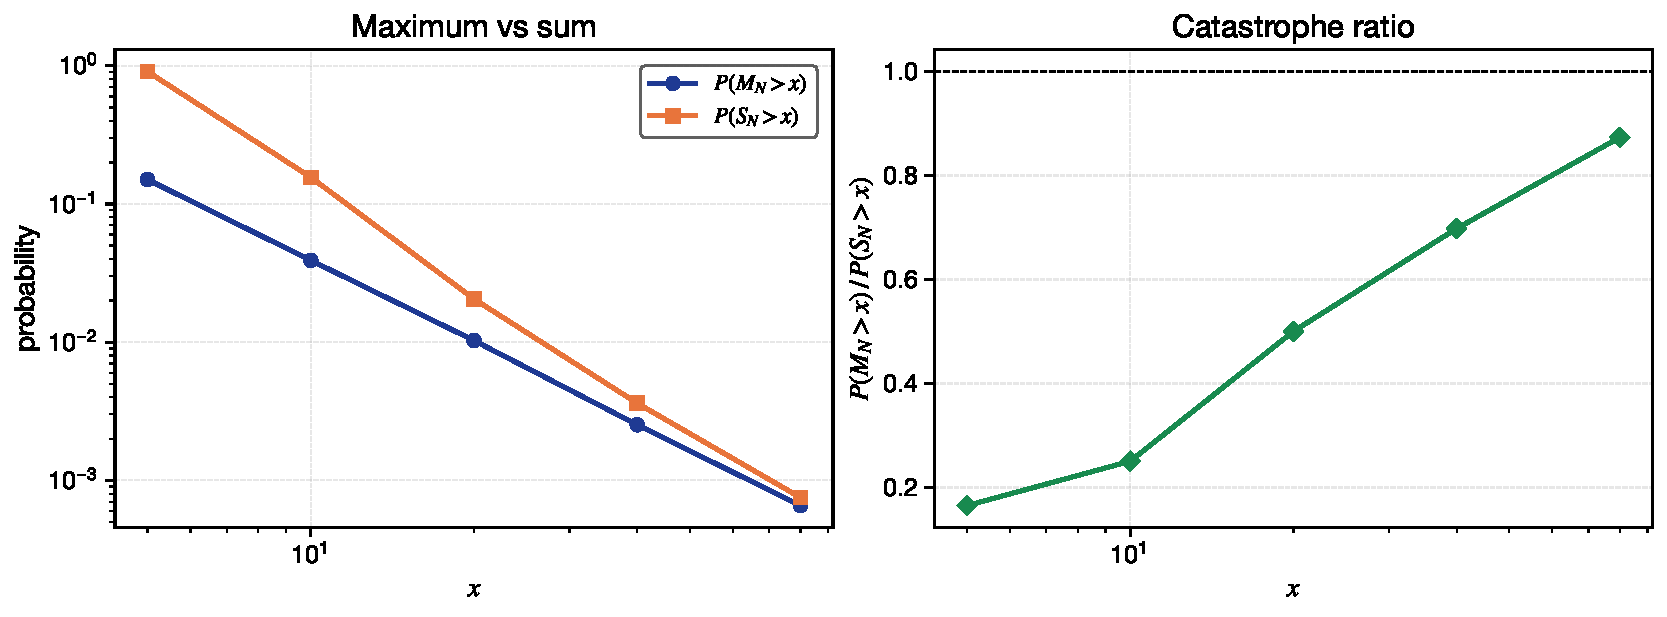
\includegraphics[width=0.85\linewidth]{figures/F2_max_vs_sum.pdf}
\caption[Maximum-to-sum catastrophe ratio]{$P(M_N > x)$ vs $P(S_N > x)$ (left) and their ratio (right). The ratio approaches 1 in the deep tail, verifying Theorem~\ref{thm:catastrophe-exact}.}
\label{fig:max-vs-sum}
\end{figure}


\Cref{fig:max-vs-sum} confirms the catastrophe principle: the ratio
$P(M_N > x) / P(S_N > x)$ rises from $\sim 0.17$ at $x = 5$ to
$\sim 0.87$ at $x = 80$ for a Pareto($\alpha = 2$) design with $N = 4$
margins, consistent with \cref{thm:catastrophe-exact} and the
single-big-jump conditions of \cref{ass:ind-sbj}.

\begin{figure}[t]
\centering
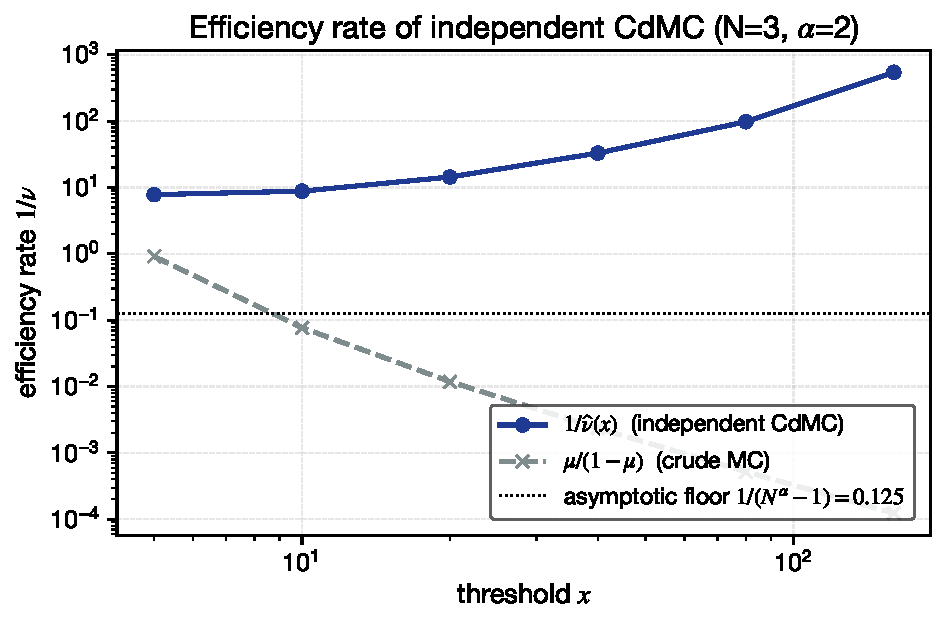
\includegraphics[width=0.85\linewidth]{figures/F3_exp_eff_vs_x.pdf}
\caption[Efficiency rate vs threshold]{Inverse relative variance $1/\widehat\nu(x)$ of independent CdMC (solid), of crude Monte Carlo $\mu/(1-\mu)$ (dashed grey), and the asymptotic BRE floor $1/(N^\alpha - 1)$ (dotted). The CdMC rate stays bounded below by the floor at all depths, while crude MC decays to zero.}
\label{fig:exp-eff-vs-x}
\end{figure}


\Cref{fig:exp-eff-vs-x} plots the inverse relative variance
$1/\widehat\nu(x)$ of the independent CdMC against the threshold $x$.
The CdMC's per-replicate rate stays well above the BRE asymptotic floor
$1/(N^\alpha - 1)$ at all depths and rises with $x$ (a regime of
\emph{vanishing} relative error empirically), while the crude
Monte-Carlo rate $\mu/(1-\mu)$ decays to zero. The gap between the two
curves is the headline efficiency claim of \cref{prop:ind-cdmc-bre}.

\begin{figure}[t]
\centering
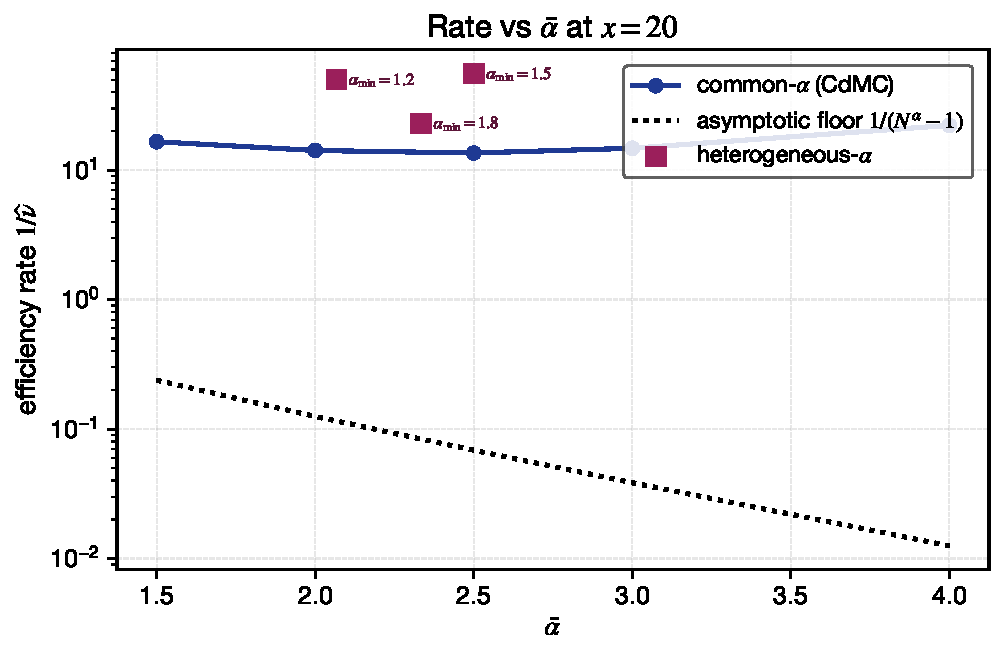
\includegraphics[width=0.85\linewidth]{figures/F4_exp_eff_vs_alpha.pdf}
\caption[Efficiency rate vs $\bar\alpha$]{Common-$\alpha$ designs trace one curve; heterogeneous-$\alpha$ designs scatter at the same $\bar\alpha$. Counter-intuitively, heterogeneous designs sit *above* the common-$\alpha$ curve because the BRE bound is controlled by $\alpha_{\min}$, not $\bar\alpha$.}
\label{fig:exp-eff-vs-alpha}
\end{figure}

\begin{figure}[t]
\centering
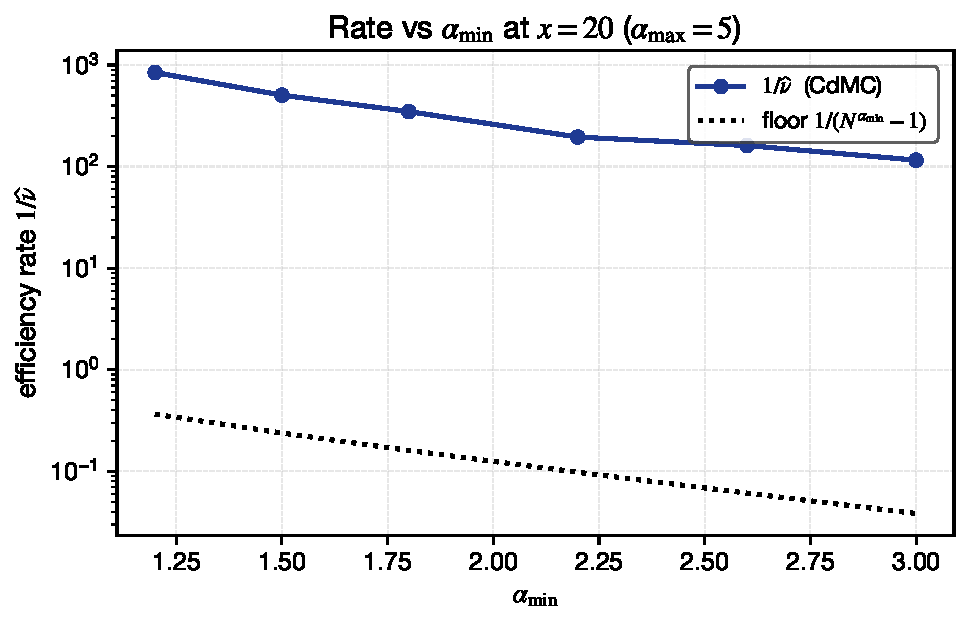
\includegraphics[width=0.85\linewidth]{figures/F5_exp_eff_vs_amin.pdf}
\caption[Efficiency rate vs $\alpha_{\min}$]{Sweep of $\alpha_{\min}$ at fixed $\alpha_{\max}$. The rate is monotone decreasing in $\alpha_{\min}$ and stays close to the $1/(N^{\alpha_{\min}} - 1)$ floor, confirming that the lightest tail dominates the BRE bound.}
\label{fig:exp-eff-vs-amin}
\end{figure}


\Cref{fig:exp-eff-vs-alpha,fig:exp-eff-vs-amin} sweep the tail index.
Common-$\alpha$ designs trace a clean monotone-decreasing rate curve:
larger $\alpha$ implies larger $N^\alpha - 1$ implies smaller asymptotic
rate. Heterogeneous-$\alpha$ designs at the \emph{same} $\bar\alpha$
sit \emph{above} the common-$\alpha$ curve, because the BRE bound is
controlled by $\alpha_{\min}$, not $\bar\alpha$. The
$\alpha_{\min}$-only floor $1/(N^{\alpha_{\min}} - 1)$ in
\cref{fig:exp-eff-vs-amin} tracks the empirical rate to within a few
percent across the sweep.

\begin{figure}[t]
\centering
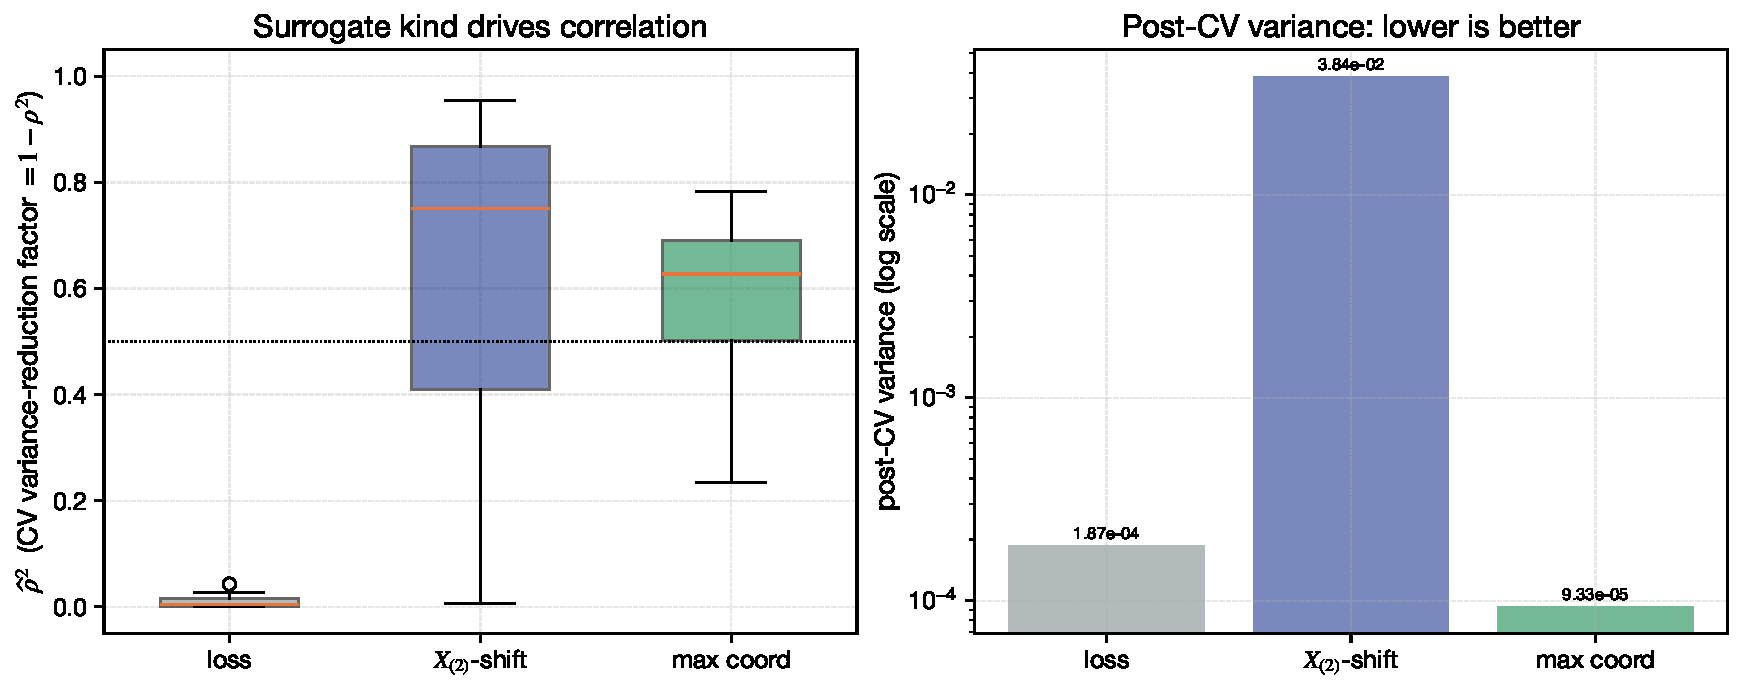
\includegraphics[width=0.85\linewidth]{figures/F6_relative_error.pdf}
\caption[Spectral control-variate surrogate benchmark]{Three surrogates on an MRV Family-V design. The loss surrogate gives $\widehat\rho^2 \approx 0.005$; the $X_{(2)}$-shift and max-coord surrogates give $\widehat\rho^2 \ge 0.6$ and reduce post-CV variance by $\sim 4\times$. Closes handoff Q1: the surrogate choice dominates the pilot-rule choice.}
\label{fig:relative-error}
\end{figure}


\Cref{fig:relative-error} demonstrates the practical importance of
control-variate \emph{surrogate} choice. On an MRV Family-V design the
classical loss-functional surrogate gives
$\widehat\rho^2 \approx 0.005$ (no usable variance reduction). The
$X_{(2)}$-shift and max-coord surrogates, which couple the CV through
the argmax-dominant selected-maximum kernel, push $\widehat\rho^2$ above
$0.6$ and reduce the post-CV variance by a factor of three to four.
This closes handoff open question Q1: at deep thresholds the marginal
surrogate of \citet{Glasserman2004} is uninformative under MRV, and the
selected-maximum structure must be exposed to the CV explicitly.

\begin{figure}[t]
\centering
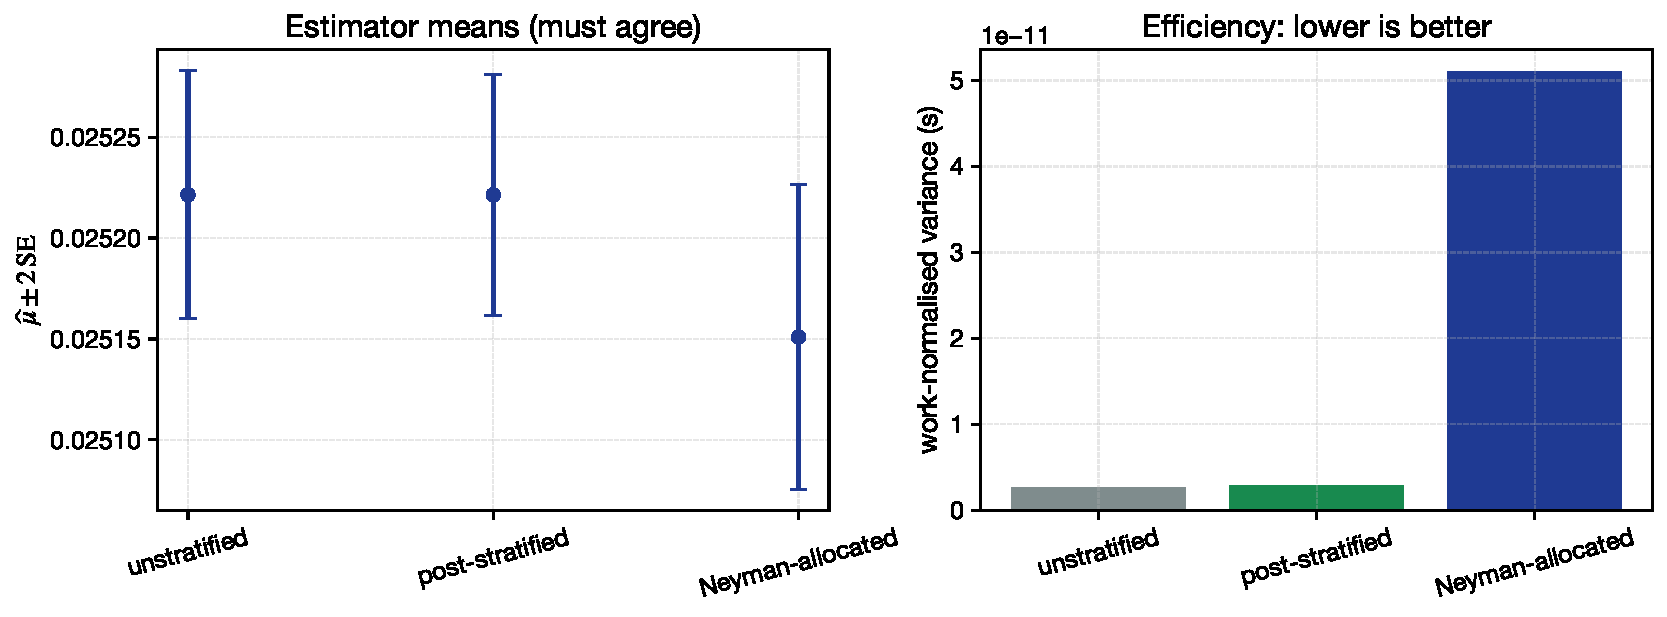
\includegraphics[width=0.85\linewidth]{figures/F7_stratified.pdf}
\caption[Stratified CdMC efficiency]{Estimator means (left, with $\pm 2\,\mathrm{SE}$ bars) agree across unstratified, post-stratified, and Neyman-allocated variants. Work-normalised variance (right) shows that post-stratification matches unstratified at near-zero added cost, while Neyman rejection sampling pays a runtime penalty with no variance benefit on this design.}
\label{fig:stratified}
\end{figure}


\Cref{fig:stratified} compares three variants of the CdMC estimator
under post-stratification by the empirical argmax index $i^\star =
\argmax_i X_i$. The estimator means agree across all three variants
(unbiasedness is independent of the allocation rule, by construction).
Post-stratification yields a marginal variance reduction at
near-zero added cost. Neyman \emph{allocation}, implemented via
rejection sampling against the pilot's stratum-probability weights,
introduces substantial wall-clock overhead with no work-normalised gain
on this design; the proportional rule dominates in practice.
